\documentclass[11pt]{article}
\usepackage{amsmath, amssymb, amsthm}
\usepackage[retainorgcmds]{IEEEtrantools}

\usepackage[pdftex]{graphicx}
\usepackage{tikz}
\usetikzlibrary{intersections}

\usepackage{fancyhdr}

%Listings stuff
\usepackage{listings}
\usepackage{lstautogobble}
\usepackage{color}

\definecolor{gray}{rgb}{0.5,0.5,0.5}
\lstset{
basicstyle={\small\ttfamily},
tabsize=3,
numbers=left,
numbersep=5pt,
numberstyle=\tiny\color{gray},
stepnumber=2,
breaklines=true,
boxpos=t
}

%Format stuff
\pagestyle{fancy}
\headheight 35pt

%Header info
\chead{\Large \textbf{Automata}}
\lhead{}
\rhead{}

\begin{document}
\section{Finite Automata}
	A finite automata is an abstract machine that starts in an initial state, and repeats some task until it ends up in a final state. An automata may have 0 or more end states but only a single start state. When using an automata to implement regex matching, the validity of a string is determined by whether or not the ending state of the automata after parsing is the final state.
	
	It is possible for an automata to have a \textbf{dead state}, that is a non-final state with no possibility of exiting. Most cases these dead states will be omitted from diagrams, so it is safe to assume that any nonexistant edges all lead to a dead state.
	
	\begin{center}
	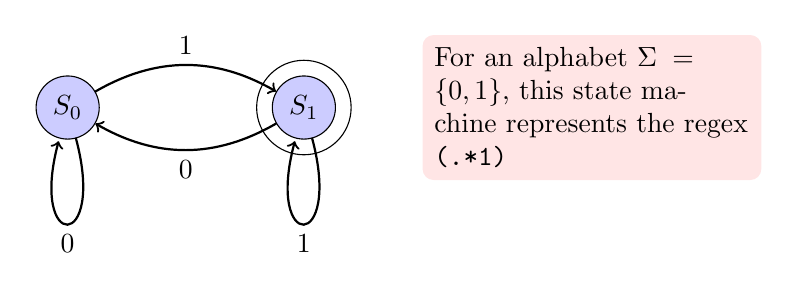
\begin{tikzpicture}
		[scale=3,line cap=round,
		%Styles
		axes/.style=,
		important line/.style={very thick},
		information text/.style={rounded corners,fill=red!10,inner sep=1ex},
		dot/.style={circle,inner sep=1pt,fill,label={#1},name=#1}	,
		main node/.style={circle,fill=blue!20,draw}		
		]
		
		%Colors
		\colorlet{anglecolor}{green!50!black}	%angle arcs/lines
		
		%The graphic
		\node[main node] (S0) at (0,0) {$S_0$};
		\node[main node] (S1) at (1, 0) {$S_1$};
		\draw (1, 0) circle (.2cm);
		
		\path 	(S0)	edge [bend left,->,thick] node[above]{$1$}	(S1)
							edge [loop below,->,thick] node[below]{$0$} (S0)
				(S1)	edge [bend left,->,thick] node[below]{$0$} (S0)
						edge [loop below,->,thick] node[below]{$1$} (S1);
							
		\draw[xshift=1.5cm]
			node[information text,right,text width=4cm] {For an alphabet $\Sigma = \{0,1\}$, this state machine represents the regex \verb|(.*1)|};
	\end{tikzpicture}
	\end{center}
	
\section{Deterministic Finite Automata}
	A DFA cannot have more than one transition leaving a state on the same symbol. A DFA will always produce the exact same path for any given string. A DFA formally is a 5-tuple $(Q, \Sigma, \delta, q_0, F)$.
	\begin{itemize}
		\item $Q$: Finite, non-empty set of states
		\item $\Sigma$: Input alphabet
		\item $\delta$: A transition function $\delta : Q\times \Sigma \rightarrow Q$
		\item $q_0$: A state state $q_0 \in Q$
		\item $F$: A set of final states $F \subset Q$
	\end{itemize}
	
\section{Nondeterministic Finite Automata}
	An NFA can have multiple multiple paths leaving a state encoded with the same symbol. An NFA will yield many possible paths for a given string, and determining the validity of a string requires a backtracking graph search. Formally, an NFA is a 5-tuple $(Q, \Sigma, \Delta, q_0, F)$ with $\Delta : Q \times \Sigma \rightarrow P(Q)$ where $P(Q)$ is the powerset of $Q$.
	
	\subparagraph{NFA-$\epsilon$} An NFA-$\epsilon$ has one or more paths encoded as an empty character, meaning that when reading through string it is possible to take a path without actually advancing a character.
	
\section{NFA - DFA Reduction}
	An NFA may be reduced to a DFA by explicitly tracking the set of NFA states. Intuitively, build a DFA where each DFA state represents a set of NFA states.
	\begin{center}
	\begin{tabular}{cc}
		NFA & DFA\\\hline
		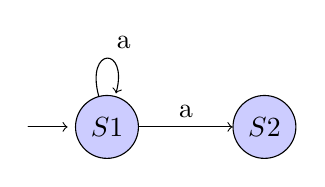
\begin{tikzpicture}
			[scale=1,line cap=round,
			%Styles
			axes/.style=,
			important line/.style={very thick},
			information text/.style={rounded corners,fill=red!10,inner sep=1ex},
			dot/.style={circle,inner sep=1pt,fill,label={#1},name=#1},
			main node/.style={circle,fill=blue!20,draw}
			]
			
			%Colors
			\colorlet{anglecolor}{green!50!black}	%angle arcs/lines
			
			%The graphic
			\node[main node] (S1) at (0,0) {$S1$};
			\node[main node] (S2) at (2,0) {$S2$};
			
			\path	(S1)	edge[->] node[above]{a} (S2)
							edge[->,loop above] node[above right] {a} (S1);
			\draw[->] (-1,0) -- (-.5,0);
		\end{tikzpicture}
		&
		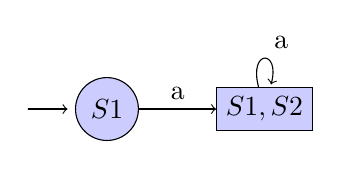
\begin{tikzpicture}
			[scale=1,line cap=round,
			%Styles
			axes/.style=,
			important line/.style={very thick},
			information text/.style={rounded corners,fill=red!10,inner sep=1ex},
			dot/.style={circle,inner sep=1pt,fill,label={#1},name=#1},
			main node/.style={circle,fill=blue!20,draw}			
			]
			
			%Colors
			\colorlet{anglecolor}{green!50!black}	%angle arcs/lines
			
			%The graphic
			\node[main node] (S1) at (0,0) {$S1$};
			\node[rectangle,fill=blue!20,draw] (S2) at (2,0) {$S1,S2$};
			
			\draw[->] (-1,0) -- (-.5,0);
			\path	(S1)	edge[->] node[above] {a} (S2)
					(S2)	edge[->,loop above] node[above right] {a} (S2);
		\end{tikzpicture}
	\end{tabular}
	\end{center}
	
	\begin{lstlisting}[autogobble=true,mathescape]
		def move(p, a):
			# p is an NFA state and a is a symbol transition
			return {q for q in NFA if <p, a, q> $\in \delta$}
			
		def reduction(NFA($\Sigma$, Q, q_0, F_n, $\delta$)):
			r_0 = {q_0}, R = {{r_0}}
			while unvisited state r in R:
				visit(r)
				for a in $\Sigma$:
					new_state = {s for s in (move(q, a) for q in r)}
					if S not in R:
						R += {S}
					$\delta$ += {<r, a, S>}
			F_d = {r for r in R if (s in r for s in F_n)}
	\end{lstlisting}
	
\section{DFA Minimization}
	Hopcroft's algorithm for DFA minimization is based on partition refinement, where DFA states are grouped into partitions by behavior. Partitions represent equivalence classes such that for any word $w$, following the transitions from two partitions $p_1, p_2$ should lead to an accepting or non-accepting state for both starting points.
	
	Partitions are split if members have transitions to different partitions for the same input word. States in the same partition should transition to the same partition for all symbols in $\Sigma$.
	
	\begin{lstlisting}[autogobble=true,mathescape]
		def minimize(DFA($\Sigma$, Q, q_0, F_n, $\delta$)):
			p_0 = F_n, p_1 = Q - F_n	# Initial partitions
			R = {p if p in (p_0 + p_1) and not p.empty}
			P = {}
			
			while P != R:
				P, R = R, {}	# P<-prev partition, R<-current
				for p in P:
					{p_0, p_1} = split(p, P)
					R += {p if p in (p_0 + p_1) and not p.empty}
					
			r_0 = R.each{|p| q_0 in p}
			F_d = {p if p in R and any([s in p for s in F_n])}
			d = q if ($\delta$(s,c) = r for s in p) and r in q
			
			return <$\Sigma$, R, r_0, F_d, d>
			
		def split(p, P):
			choose r from p
			q = p - {r}, m = {}
			
			for s in q:
				for c in $\Sigma$:
					if ($\delta$(r,c) = q_0 and $\delta$(s,c) = q_1) and 
						not any(
							(q_0 in p_1 and q_1 in p_1) for p_1 in P)
						m += {s}
			
			# m are states that behave differently than r
			# p-m are states that behave the same as r
			return p-m, m 
	\end{lstlisting}
	
\section{DFA Complement}
	Given a DFA accepting a language $L$, the DFA accepting its complement is simply the DFA with every accepting state flipped to a non-accepting state and every non-accepting state to an accepting state. Note that this \textbf{only} works with DFA's.

%	\begin{center}
%	\begin{tikzpicture}
%		[scale=3,line cap=round,
%		%Styles
%		axes/.style=,
%		important line/.style={very thick},
%		information text/.style={rounded corners,fill=red!10,inner sep=1ex},
%		dot/.style={circle,inner sep=1pt,fill,label={#1},name=#1}			
%		]
%		
%		%Colors
%		\colorlet{anglecolor}{green!50!black}	%angle arcs/lines
%		
%		%The graphic
%	\end{tikzpicture}
%	\end{center}

%	\begin{figure}[htb]
%		\centering
%		\includegraphics[width=0.8\textwidth]{filename.eps}
%		\caption{Caption.}
%		\label{fig:figure}
%	\end{figure}

%		\def\enotesize{\normalsize}
%		\theendnotes
\end{document}